\documentclass[dvipsnames]{beamer}

\usepackage{xcolor}
\usepackage{lmodern}
\usepackage{minted}
\usepackage[utf8]{inputenc}
\usepackage{standalone}
\usepackage{tikz}
\usepackage{caption}
\usepackage{adjustbox}
\usepackage{upquote}
\usepackage{hyperref}
\usepackage{multirow}
\usepackage{booktabs}
\usepackage{array}
\usepackage{xspace}

\usetikzlibrary{mindmap,shadows,arrows,positioning,chains,fit,shapes}

\usetheme{metropolis}
\usemintedstyle{manni}

\definecolor{gmitblue}{RGB}{20,134,225}
\definecolor{gmitred}{RGB}{220,20,60}
\definecolor{gmitgrey}{RGB}{67,67,67}

\setbeamercolor{structure}{fg=gmitblue}
\setbeamercolor{frametitle}{fg=white, bg=gmitred}
\setbeamercolor{alerted text}{fg=gmitblue}

\renewcommand\footnoterule{}
\newcommand{\citeurl}[1]{\let\thefootnote\relax\footnotetext{\tiny \textcolor{gmitgrey}{\href{http://#1}{#1}}}}

\newcommand{\hr}{\rule{\textwidth}{0.5pt}}

\makeatletter
\expandafter\def\csname PYGdefault@tok@err\endcsname{\def\PYGdefault@bc##1{{\strut ##1}}}
\makeatother

\begin{document}
  \title{Data Representation and Querying}
  \subtitle{}
  \author{ian.mcloughlin@gmit.ie}
  \date{}

  \begin{frame}
    \titlepage
  \end{frame}

  \begin{frame}
    \frametitle{Topics}
    \tableofcontents
  \end{frame}

  %!TEX root = ../slides.tex
\section{HTTP}


\begin{frame}{HyperText Transfer Protocol}
  \begin{description}
		\item[HyperText] Text with links.
		\item[Transfer] Communication of data.
		\item[Protocol] Set of rules for communication.\\[1cm]
    \item[HTTP/1.0] was the first version.
    \item[HTTP/1.1] is the current widely used version.
    \item[HTTP/2] use is slowly growing.
  \end{description}
\end{frame}


\begin{frame}{Why study HTTP?}
  \begin{description}
		\item[HTTP] is the main protocol used by web browsers.
    \item[Netflix] uses HTTP to stream video (using DASH).
    \item[Instagram] is basically just a HTTP API.
    \item[Facebook] is a web application using HTTP.
    \item[GMail] uses HTTP.
    \item[Twitter] uses HTTP.
    \item[Medium] is really clever about its use of HTTP.
    \item[Sandvine] suggest most internet traffic happens over HTTP.  
  \end{description}
  \citeurl{sandvine.com/downloads/general/global-internet-phenomena/2015}
\end{frame}


\begin{frame}{Why is HTTP so widely used?}
  \begin{description}
		\item[HTTP] is often used instead of protocols that are more suited to the application.
    \item[Browsers] are one of the main reasons for this. Modern operating systems come with one or more browsers installed by default.
    \item[Web servers] and browsers mainly talk over HTTP.
    \item[Libraries] exist for most programming languages to make HTTP requests.
    \item[HTTP] is relatively straght-forward.
    \item[Firewalls] usually do not block HTTP by default.  
  \end{description}
\end{frame}


\begin{frame}{What is HTTP?}
  \begin{description}
		\item[You] will know HTTP from typing \mintinline{http}{http://} in your browser's location bar.
    \item[RFC 2616] details HTTP/1.1.
    \item[HTTP] is a standard way of transmitting data at the application level.
    \item[Originally] it was for transmitting text.
    \item[Text] is strings of ones and zeroes chopped into chunks, where each chuck represents a letter or character.
    \item[Nothing] stops us from sending non-text data via HTTP. 
  \end{description}
\end{frame}


\begin{frame}{How does HTTP work?}
  \begin{description}
		\item[Clients] performs requests. Firefox is an example of a client.
    \item[Servers] respond to requests. Apache is an example of a server.
    \item[Requests] are text documents sent by clients to servers.
    \item[Responses] are text documents sent by server to clients.
    \item[URLs] specify the server's location and the resource on the server.
    \item[Headers] are text metadata added to the start of requests and responses.
    \item[Bodies] are the main content of responses, and sometimes requests.
    \item[HTML] typically forms the body of a response.  
  \end{description}
\end{frame}


\begin{frame}{Request--Response}
  \tikzstyle{rect} = [rectangle,fill=gmitblue,text width=4.5em,text centered,minimum height=4em,rounded corners,text=white]
  \tikzstyle{line} = [draw,->,very thick]
  \tikzstyle{oval} = [ellipse,fill=gmitred,text width=5em,text centered,text=white]
  \begin{adjustbox}{max width={0.9\textwidth},center} 
    \begin{tikzpicture}[node distance = 4cm]
      \node [oval] (client1) {Client (Firefox)};
      \node [rect, right of=client1] (request) {Request};
      \node [rect, right of=client1] (request) {Request};
      \node [oval, right of=request] (server1) {Server (Apache)};
      \node [rect, below=1cm of server1] (generate) {Generate response};
      \node [oval, below=1cm of generate] (server2) {Server (Apache)};
      \node [rect, left of=server2] (response) {Response};
      \node [oval, left of=response] (client2) {Client (Firefox)};
      \path [line] (client1) -- (request);
      \path [line] (request) -- (server1);
      \path [line,dashed] (server1) -- (generate);
      \path [line,dashed] (generate) -- (server2);
      \path [line] (server2) -- (response);
      \path [line] (response) -- (client2);
    \end{tikzpicture}
  \end{adjustbox}
\end{frame}


\begin{frame}{HTTP is not like a phone call}
  \begin{description}
		\item[Suppose] I ring you and ask for your PPS Number.
    \item[If] you don't understand the question, you can say ``Sorry, can you please repeat that?''.
    \item[Then] I repeat my question, and you then give me the number before hanging up.\\[1cm]
    \item[HTTP] doesn't work like that.
    \item[Misunderstandings] result in the server responding with an error, and hanging up.
    \item[Status codes] indicate errors, amongst other things.
  \end{description}
\end{frame}


\begin{frame}{Uniform Resource Locator}
  \textcolor{BlueViolet}{http}://%
  \textcolor{RubineRed}{username}:%
  \textcolor{Mahogany}{password}@%
  \textcolor{MidnightBlue}{www}.%
  \textcolor{OliveGreen}{reddit.com}:%
  \textcolor{Dandelion}{80}%
  \textcolor{Plum}{/r/funny/}?%
  \textcolor{DarkOrchid}{limit=1}
  
  \begin{table}
    \begin{tabular}{r@{\hspace{0.5cm}}p{6cm}}
      \textcolor{BlueViolet}{http} & Protocol \\
      \textcolor{RubineRed}{username} & Username \\
      \textcolor{Mahogany}{password} & Password \\
      \textcolor{MidnightBlue}{www} & Subdomain \\
      \textcolor{OliveGreen}{reddit.com} & Domain \\
      \textcolor{Dandelion}{80} & Port \\
      \textcolor{Plum}{/r/funny/} & Path \\
      \textcolor{DarkOrchid}{limit=1} & Parameter
    \end{tabular}
  \end{table}
\end{frame}


\begin{frame}[fragile]{Request and Response Format}
  Requests and responses both have this format:
  \begin{itemize}
    \item Intial line.
    \item Zero or more header lines.
    \item A blank line.
    \item Optional message body (e.g. a HTML file)
  \end{itemize}
  \citeurl{www.jmarshall.com/easy/http}
\end{frame}


\begin{frame}[fragile]{Request (GET) Example}
  \begin{minted}{http}
GET /courses/all-courses HTTP/1.1
Host: gmit.ie
User-Agent: curl/7.50.1
Accept: */*

  \end{minted}
\end{frame}

\begin{frame}[fragile]{Response Example}
  \begin{minted}{http}
HTTP/1.1 200 OK
Date: Mon, 27 Jul 2009 12:28:53 GMT
Server: Apache/2.2.14 (Win32)
Last-Modified: Wed, 22 Jul 2009 19:15:56 GMT
Content-Length: 88
Content-Type: text/html
Connection: Closed

<html>
  <body>
    <h1>Hello, World!</h1>
  </body>
</html>
  \end{minted}
\end{frame}


\begin{frame}{Resources}
 \begin{columns}[onlytextwidth]
   \begin{column}{0.5\textwidth}
     \centering
      \begin{figure}
        
\begin{tikzpicture}
          \draw (0,0) -- (0,1.2) -- (0.7,1.2) -- (0.7,0.8) -- (1,0.8) -- (1,0) -- cycle;
          \draw (0.7,1.2) -- (1,0.8);
        \end{tikzpicture}
        \caption*{File}
      \end{figure}
    \end{column}
    \begin{column}{0.5\textwidth}
      \centering
      \begin{figure}
      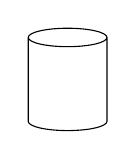
\begin{tikzpicture}
        \node (A) [cylinder, shape border rotate=90, draw,minimum height=1.3cm,minimum width=1cm] {};
      \end{tikzpicture}
      \caption*{Database}
      \end{figure}
    \end{column}
  \end{columns}
  
  \begin{quote}
    HTTP is used to transmit resources \ldots A resource is some chunk of information that can be identified by a URL \ldots The most common kind of resource is a file, but a resource may also be a dynamically-generated query result \ldots
  \end{quote}
  \citeurl{www.jmarshall.com/easy/http}
\end{frame}


\begin{frame}{HTTP Methods}
  \begin{description}
    \item[GET] Retrieve information from the server.
    \item[HEAD] Like get, but retrieve only the response header.
    \item[POST] Send data to the server.
    \item[PUT] Set the resource at the URL to the request data.
    \item[DELETE] Delete the resource at the URL.
    \item[CONNECT] Set up tunnel for other traffic to pass through HTTP.
    \item[OPTIONS] Find the allowable operations at the given URL.
    \item[TRACE] Echo the received request.
    \item[PATCH] Partial resource modification.
  \end{description}
\end{frame}


\begin{frame}{Status codes}
  \begin{description}
    \item[404] is probably the most famous status code. It means you requested a resource that doesn't exist on the server.
    \item[200] means everything is OK, and is the most common one in everyday browsing.
    \item[All] status codes are three digit numbers.
    \item[1xx] indicates an informational message only
    \item[2xx] indicates success of some kind
    \item[3xx] redirects the client to another URL
    \item[4xx] indicates an error on the client's part
    \item[5xx] indicates an error on the server's part
  \end{description}
  \citeurl{www.jmarshall.com/easy/http}
\end{frame}


\begin{frame}{Sending data to the server}
  \begin{description}
    \item[Sometimes] we want to tell the server something extra.
    \item[Resources] can be generated differently based on this extra data.
    \item[Google] can use this to perform searches on google.ie
    \item[Try] opening \mintinline{http}{google.ie} in your browser, and then open \mintinline{http}{google.ie/?q=gmit}.
    \item[The requested] resource here is the same but we don't get the same response.
    \item[Two] main ways to send extra data to the server: in the URL after a question mark, or in the body of the request.
  \end{description}
  \citeurl{www.jmarshall.com/easy/http}
\end{frame}


\begin{frame}{URL encoding}
  HTML form data is usually URL-encoded by changing:
  \begin{itemize}
    \item Unsafe characters to \% \emph{xx} where \emph{xx} is the ASCII value.
    \item All spaces to plusses.
    \item Names and values to: name1=value1\&name2=value2.
  \end{itemize}
  \hr
  \begin{description}
    \item[GET] --- in the URL after a question mark.
    \item[POST] --- in the body.
  \end{description}
  \citeurl{www.jmarshall.com/easy/http}
\end{frame}

\begin{frame}[fragile]{Request (GET) with parameters}
  \begin{minted}{http}
GET /r/ireland?limit=1 HTTP/1.1
Host: reddit.com
User-Agent: curl/7.50.1
Accept: */*

  \end{minted}
\end{frame}


\begin{frame}[fragile]{Request (POST) Example}
  \begin{minted}{http}
POST /path/script.cgi HTTP/1.0
From: frog@jmarshall.com
User-Agent: HTTPTool/1.0
Content-Type: application/x-www-form-urlencoded
Content-Length: 32

home=Cosby&favorite+flavor=flies
  \end{minted}
\end{frame}

  %!TEX root = ../slides.tex
\section{Data}


\begin{frame}{JSON}
  \begin{description}
    \item[JavaScript] A scripting/programming language.
    \vspace{0.25cm}
    \item[Object] Groups of name--value pairs.
    \vspace{0.25cm}
    \item[Notation] Set of rules for representing objects.
  \end{description}
  \begin{itemize}
    \item JSON is just text --- text that conforms to a syntax.
    \item JSON is heavily influenced by JavaScript, but it is used in with all languages.
    \item JSON's primary purpose is to represent information in text form.
    \item JSON is popular because it is easy to send over HTTP and parse in JavaScript.
  \end{itemize}
\end{frame}

\begin{frame}{Sending JSON}
  \tikzstyle{block} = [rectangle, fill=azure(colorwheel), text width=4.5em, text centered, minimum height=4em]
  \tikzstyle{line} = [draw, -latex']
  \tikzstyle{cloud} = [ellipse, fill=wildwatermelon, text width=5em, text centered]
  \tikzstyle{startstop} = [rectangle, rounded corners, text width=5em, minimum height=4em, text centered, fill=tiffanyblue]
  
  \begin{adjustbox}{max totalsize={.9\textwidth}{.6\textheight},center}
  
  \tikzstyle{rect} = [rectangle,fill=gmitblue,text width=4.5em,text centered,minimum height=4em,rounded corners,text=white]
  \tikzstyle{line} = [draw,->,very thick]
  \tikzstyle{oval} = [ellipse,fill=gmitred,text width=5em,text centered,text=white]
    
    \begin{tikzpicture}[node distance=4cm]
    \node [oval] (object1) {Object Instance};
    \node [rect, below of=object1] (json1) {JSON};
    \node [rect, right of=json1, node distance = 6cm] (json2) {JSON};
    \node [oval, above of=json2] (object2) {Object Instance};
    % Draw edges
    \path [line] (object1) -- node[style={rectangle,fill=white,draw}]{stringify} (json1);
    \path [line] (json1) -- node[style={rectangle,fill=white},draw ]{HTTP} (json2);
    \path [line] (json2) -- node[style={rectangle,fill=white,draw}]{parse} (object2);
    % Draw Memory
    \draw [color=gray, dashed](-2,-1.5) rectangle (2,1.25);
    \node at (-1.4,-1.35) [] {\tiny Machine 1};
    \draw [color=gray, dashed](4,-1.5) rectangle (8,1.25);
    \node at (4.6,-1.35) [] {\tiny Machine 2};
    \end{tikzpicture}
  \end{adjustbox}
\end{frame}

\begin{frame}[fragile]{JSON Example}
  \begin{minted}{json}
{
  "employees": [
    {"firstName":"John", "lastName":"Doe"},
    {"firstName":"Anna", "lastName":"Smith"},
    {"firstName":"Peter", "lastName":"Jones"}
  ]
}
  \end{minted}
\end{frame}


\begin{frame}[fragile]{Using JSON in JavaScript}
  \begin{minted}{javascript}
// Turning text into a JavaScript object.
var obj = JSON.parse(text);
// obj is an obect.

// Turning a JavaScript object into text.
var text = JSON.stringify(obj);
// text is a string.
  \end{minted}
\end{frame}

\begin{frame}{JSON Syntax}
  \begin{itemize}
    \item Name/Value pairs separated by a colon. \\
    \hspace{0.5cm} \mintinline{json}{"name": "Ian"}
    \item Objects identified by curly braces. \\
    \hspace{0.5cm} \mintinline{json}{{}}
    \item Lists identified by square brackets. \\
    \hspace{0.5cm} \mintinline{json}{[]}
    \item All strings (and names) use double quotes (not single). \\
    \hspace{0.5cm} \mintinline{json}{"Ian"}
  \end{itemize}
\end{frame}

\begin{frame}{JSON Types}
  \begin{itemize}
    \item Numbers \\
    \hspace{0.5cm} \mintinline{json}{123.456}
    \item Strings \\
    \hspace{0.5cm} \mintinline{json}{"Hello, world!"}
    \item Boolean \\
    \hspace{0.5cm} \mintinline{json}{true"}
    \item Arrays\\
    \hspace{0.5cm} \mintinline{json}{[1,2,3]}
    \item Objects\\
    \hspace{0.5cm} \mintinline{json}{{"name": "Ian"}}
    \item null \\
    \hspace{0.5cm} \mintinline{json}{null}
  \end{itemize}
\end{frame}



\begin{frame}{eXtensible Markup Language}
  \begin{description}
    \item[Extensible] Designed to accommodate change.
    \vspace{0.25cm}
    \item[Markup] Annotates text.
    \vspace{0.25cm}
    \item[Language] Set of rules for communication.
  \end{description}
\end{frame}


\begin{frame}{About XML}
  \begin{itemize}
    \item XML is an alternative to JSON.
    \item XML looks like HTML, but it is different.
    \item XML's purpose is to represent information in text form.
    \item There are no pre-defined tag names -- you make them up yourself.
    \item XML has a tree-like syntax.
    \item The Document Object Model (DOM) can be applied to XML.
  \end{itemize}
\end{frame}


\begin{frame}[fragile]{XML Example}
  \begin{minted}{xml}
<?xml version="1.0" encoding="UTF-8"?>
<book isbn-13="978-0131774292" isbn-10="0131774298">
  <title>Expert C Programming: Deep C Secrets</title>
  <publisher>Prentice Hall</publisher>
  <author>Peter van der Linden</author>
</book>
  \end{minted}
\end{frame}

\begin{frame}{XML Syntax}
  \begin{description}
    \item[Declaration] XML documents should have a single line at the start stating that it's XML, the version of XML it is, and an encoding.
    \item[Elements] XML is structured as elements, which are enclosed in angle brackets.
    \item[Root element] XML must have a single root element that wraps all others.
    \item[Attbirutes] Elements can have attributes, which are name--value pairs within the angle brackets. A given attribute name can only be specified once per element.
    \item[Entity references] Certain characters must be escaped with entity references, e.g.\ \&lt; for $\langle$.
    \item[Case sensitive] Everything in XML is case sensitive.
  \end{description}
\end{frame}

\begin{frame}[fragile]{XML Syntax Example}
  \begin{minted}{xml}
  <?xml version="1.0" encoding="UTF-8"?>
  <parent-element attribute-name="attribute-value">
    <child name="value">Text</child-element>
    <child name="value">Text</child-element>
    <child name="value">Text</child-element>
    <lone-warrior />
  </parent-element>
  \end{minted}
\end{frame}

\begin{frame}{Document Object Model}
  \begin{itemize}
    \item The Document Object Model (DOM) is a programming interface for HTML and XML documents.
    \item It provides a model of the document as a structured group of nodes that have properties and methods.
    \item The DOM connects web pages to scripts or programming languages.
    \item You can use document.createElement, document.createTextNode and document.element.appendChild to add to the DOM.
    \item You can use document.getElementById to access elements of the DOM.
  \end{itemize}
  \citeurl{developer.mozilla.org/en-US/docs/Web/API/Document\_Object\_Model/Introduction}
\end{frame}


\begin{frame}{Asynchronous JavaScript and XML}
  AJAX stands for Asynchronous JavaScript and XML.
  \vspace{0.5cm}
  \begin{description}
    \item[Asynchronous] In the background, and without a page refresh.
    \vspace{0.25cm}
    \item[JavaScript] Programming language for the web.
    \vspace{0.25cm}
    \item[XML] eXtensible Markup Language.
  \end{description}
\end{frame}


\begin{frame}{About AJAX}
  \begin{itemize}
    \item AJAX allows us to make a HTTP request from JavaScript without a page refresh.
    \item AJAX also allows us to receive the response from that request and deal with it.
    \item Despite the name, we don't have to use XML -- we can use JSON or anything else.
    \item This happens asynchronously, so that the rest of our code be run while waiting for a slower piece of code to complete.
    \item HTTP requests are usually relatively slow.
    \item We use a callback function, which is called when the HTTP transaction is complete.
  \end{itemize}
\end{frame}


\begin{frame}[fragile]{AJAX Example}
  \begin{minted}{javascript}
var xmlhttp = new XMLHttpRequest();

xmlhttp.onreadystatechange = function() {
  if (xmlhttp.readyState == 4) {
    var mydiv = document.getElementById("mydivid");
    mydiv.innerHTML = xmlhttp.responseText;
  }
};

xmlhttp.open("GET", "https://goo.gl/2GCplC");
xmlhttp.send();
  \end{minted}
\end{frame}


\begin{frame}{AJAX Example Explained}
  \begin{itemize}
    \item XMLHttpRequest is a built-in class that provides AJAX functionality in JavaScript.
    \item httpRequest.onreadystatechange should be set to a function to run every time something happens in our HTTP call.
    \item httpRequest.open is called to initialize the request.
    \item httpRequest.send is used to send the request to the server.
    \item XMLHttpRequest.readyState changes when the state of the AJAX call changes. This triggers a call to httpRequest.onreadystatechange.
  \end{itemize}
\end{frame}


\begin{frame}[fragile]{Using jQuery}
  \begin{minted}{html}
<script src="jquery.min.js"></script>
  \end{minted}
  \vspace{1cm}
  \begin{minted}{javascript}
$.get("https://goo.gl/2GCplC", function(data) {
  $("#mydivid").html(data);
});
  \end{minted}
\end{frame}
  %!TEX root = ../slides.tex
\section{REST}


\begin{frame}{HTTP APIs}
	\begin{itemize}
		\item Facebook, Google, Reddit and others often provide programmable interfaces to their services.
		\item This lets other application developers use the services programmatically.
		\item For instance, Reddit allows developers to create mobile apps for viewing and making submissions to reddit.
		\item HTTP is often the mechanism used for this purpose.
		\item Access is provided through a set of URLs, across a variety of HTTP methods.
		\item The APIs often require JSON in HTTP request bodies and often return the query results as JSON.
	\end{itemize}
\end{frame}


\begin{frame}{REST}
  \begin{itemize}
    \item REST stands for Representational State Transfer.
    \item REST is an architecture describing how we might use HTTP.
    \item RESTful APIs make use of more HTTP methods than just GET and POST.
    \item Most HTTP APIs are not RESTful.
    \item RESTful APIs adhere to a few loosely defined constraints.
    \item Two of those constraints are that the API is stateless and cacheable.
  \end{itemize}
  \citeurl{drdobbs.com/web-development/restful-web-services-a-tutorial/240169069}
\end{frame}


\begin{frame}{HTTP and CRUD}
  \tikzset{->-/.style={decoration={markings,mark=at position .5 with {\arrow{>}}},postaction={decorate}}}
  \tikzset{-<-/.style={decoration={markings,mark=at position .5 with {\arrow{<}}},postaction={decorate}}}
  \tikzstyle{rect} = [rectangle,fill=gmitblue,text width=5em,text centered,minimum height=16em,rounded corners,text=white]
  \begin{adjustbox}{max width={0.9\textwidth},center} 
    \begin{tikzpicture}[thick]

      \node [rect] (database) at (10,0) {Database};
      \node [rect] (webserver) at (5,0) {Web \\ Server};
      \node [rect] (client) at (0,0) {Client};

      \pgfmathsetmacro{\levela}{6em}
      \pgfmathsetmacro{\levelb}{2em}
      \pgfmathsetmacro{\levelc}{-2em}
      \pgfmathsetmacro{\leveld}{-6em}
      \pgfmathsetmacro{\diff}{0.3em}

      \path ([yshift={\levela+\diff}]webserver.west) edge[<-] node[anchor=south] {\footnotesize POST}     ([yshift={\levela+\diff}]client.east);
      \path ([yshift={\levela-\diff}]webserver.west) edge[->]                                             ([yshift={\levela-\diff}]client.east);
      
      \path ([yshift={\levela+\diff}]database.west) edge[<-] node[anchor=south] {\footnotesize CREATE}    ([yshift={\levela+\diff}]webserver.east);
      \path ([yshift={\levela-\diff}]database.west) edge[->]                                              ([yshift={\levela-\diff}]webserver.east);

      \path ([yshift={\levelb+\diff}]webserver.west) edge[<-] node[anchor=south] {\footnotesize GET}      ([yshift={\levelb+\diff}]client.east);
      \path ([yshift={\levelb-\diff}]webserver.west) edge[->]                                             ([yshift={\levelb-\diff}]client.east);
      
      \path ([yshift={\levelb+\diff}]database.west) edge[<-] node[anchor=south] {\footnotesize RETRIEVE}  ([yshift={\levelb+\diff}]webserver.east);
      \path ([yshift={\levelb-\diff}]database.west) edge[->]                                              ([yshift={\levelb-\diff}]webserver.east);

      \path ([yshift={\levelc+\diff}]webserver.west) edge[<-] node[anchor=south] {\footnotesize PUT}      ([yshift={\levelc+\diff}]client.east);
      \path ([yshift={\levelc-\diff}]webserver.west) edge[->]                                             ([yshift={\levelc-\diff}]client.east);
      
      \path ([yshift={\levelc+\diff}]database.west) edge[<-] node[anchor=south] {\footnotesize UPDATE}    ([yshift={\levelc+\diff}]webserver.east);
      \path ([yshift={\levelc-\diff}]database.west) edge[->]                                              ([yshift={\levelc-\diff}]webserver.east);

      \path ([yshift={\leveld+\diff}]webserver.west) edge[<-] node[anchor=south] {\footnotesize DELETE}   ([yshift={\leveld+\diff}]client.east);
      \path ([yshift={\leveld-\diff}]webserver.west) edge[->]                                             ([yshift={\leveld-\diff}]client.east);
      
      \path ([yshift={\leveld+\diff}]database.west) edge[<-] node[anchor=south] {\footnotesize DELETE}  ([yshift={\leveld+\diff}]webserver.east);
      \path ([yshift={\leveld-\diff}]database.west) edge[->]                                              ([yshift={\leveld-\diff}]webserver.east);

      \draw ([yshift={\levela+\diff}]webserver.west)  edge[dashed,draw=gray!60,->-] ([yshift={\levela+\diff}]webserver.east);
      \draw ([yshift={\levela-\diff}]webserver.west)  edge[dashed,draw=gray!60,-<-] ([yshift={\levela-\diff}]webserver.east);
      \draw ([yshift={\levelb+\diff}]webserver.west)  edge[dashed,draw=gray!60,->-] ([yshift={\levelb+\diff}]webserver.east);
      \draw ([yshift={\levelb-\diff}]webserver.west)  edge[dashed,draw=gray!60,-<-] ([yshift={\levelb-\diff}]webserver.east);
      \draw ([yshift={\levelc+\diff}]webserver.west)  edge[dashed,draw=gray!60,->-] ([yshift={\levelc+\diff}]webserver.east);
      \draw ([yshift={\levelc-\diff}]webserver.west)  edge[dashed,draw=gray!60,-<-] ([yshift={\levelc-\diff}]webserver.east);
      \draw ([yshift={\leveld+\diff}]webserver.west)  edge[dashed,draw=gray!60,->-] ([yshift={\leveld+\diff}]webserver.east);
      \draw ([yshift={\leveld-\diff}]webserver.west)  edge[dashed,draw=gray!60,-<-] ([yshift={\leveld-\diff}]webserver.east);

      \draw[dashed,draw=gray!60] ([yshift={\levela+\diff}]database.west)  -- ([yshift={\levela+\diff}]database.center) -- ([yshift={\levela-\diff}]database.center) -- ([yshift={\levela-\diff}]database.west);
      \draw[dashed,draw=gray!60] ([yshift={\levelb+\diff}]database.west)  -- ([yshift={\levelb+\diff}]database.center) -- ([yshift={\levelb-\diff}]database.center) -- ([yshift={\levelb-\diff}]database.west);
      \draw[dashed,draw=gray!60] ([yshift={\levelc+\diff}]database.west)  -- ([yshift={\levelc+\diff}]database.center) -- ([yshift={\levelc-\diff}]database.center) -- ([yshift={\levelc-\diff}]database.west);
      \draw[dashed,draw=gray!60] ([yshift={\leveld+\diff}]database.west)  -- ([yshift={\leveld+\diff}]database.center) -- ([yshift={\leveld-\diff}]database.center) -- ([yshift={\leveld-\diff}]database.west);


    \end{tikzpicture}
  \end{adjustbox}
\end{frame}

\begin{frame}{AMP}
  \tikzset{->-/.style={decoration={markings,mark=at position .5 with {\arrow{>}}},postaction={decorate}}}
  \tikzset{-<-/.style={decoration={markings,mark=at position .5 with {\arrow{<}}},postaction={decorate}}}
  \tikzstyle{rect} = [rectangle,fill=gmitblue,text width=5em,text centered,minimum height=16em,rounded corners,text=white]
  \begin{adjustbox}{max width={0.9\textwidth},center} 
    \begin{tikzpicture}[thick]

      \node [rect] (database) at (10,0) {MySQL};
      \node [rect] (webserver) at (5,0) {Apache \\ and PHP};
      \node [rect] (client) at (0,0) {Firefox};

      \pgfmathsetmacro{\levela}{6em}
      \pgfmathsetmacro{\levelb}{2em}
      \pgfmathsetmacro{\levelc}{-2em}
      \pgfmathsetmacro{\leveld}{-6em}
      \pgfmathsetmacro{\diff}{0.3em}

      \path ([yshift={\levela+\diff}]webserver.west) edge[<-] node[anchor=south] {\footnotesize POST}     ([yshift={\levela+\diff}]client.east);
      \path ([yshift={\levela-\diff}]webserver.west) edge[->]                                             ([yshift={\levela-\diff}]client.east);
      
      \path ([yshift={\levela+\diff}]database.west) edge[<-] node[anchor=south] {\footnotesize INSERT}    ([yshift={\levela+\diff}]webserver.east);
      \path ([yshift={\levela-\diff}]database.west) edge[->]                                              ([yshift={\levela-\diff}]webserver.east);

      \path ([yshift={\levelb+\diff}]webserver.west) edge[<-] node[anchor=south] {\footnotesize GET}      ([yshift={\levelb+\diff}]client.east);
      \path ([yshift={\levelb-\diff}]webserver.west) edge[->]                                             ([yshift={\levelb-\diff}]client.east);
      
      \path ([yshift={\levelb+\diff}]database.west) edge[<-] node[anchor=south] {\footnotesize SELECT}  ([yshift={\levelb+\diff}]webserver.east);
      \path ([yshift={\levelb-\diff}]database.west) edge[->]                                              ([yshift={\levelb-\diff}]webserver.east);

      \path ([yshift={\levelc+\diff}]webserver.west) edge[<-] node[anchor=south] {\footnotesize PUT}      ([yshift={\levelc+\diff}]client.east);
      \path ([yshift={\levelc-\diff}]webserver.west) edge[->]                                             ([yshift={\levelc-\diff}]client.east);
      
      \path ([yshift={\levelc+\diff}]database.west) edge[<-] node[anchor=south] {\footnotesize UPDATE}    ([yshift={\levelc+\diff}]webserver.east);
      \path ([yshift={\levelc-\diff}]database.west) edge[->]                                              ([yshift={\levelc-\diff}]webserver.east);

      \path ([yshift={\leveld+\diff}]webserver.west) edge[<-] node[anchor=south] {\footnotesize DELETE}   ([yshift={\leveld+\diff}]client.east);
      \path ([yshift={\leveld-\diff}]webserver.west) edge[->]                                             ([yshift={\leveld-\diff}]client.east);
      
      \path ([yshift={\leveld+\diff}]database.west) edge[<-] node[anchor=south] {\footnotesize DELETE}  ([yshift={\leveld+\diff}]webserver.east);
      \path ([yshift={\leveld-\diff}]database.west) edge[->]                                              ([yshift={\leveld-\diff}]webserver.east);

      \draw ([yshift={\levela+\diff}]webserver.west)  edge[dashed,draw=gray!60,->-] ([yshift={\levela+\diff}]webserver.east);
      \draw ([yshift={\levela-\diff}]webserver.west)  edge[dashed,draw=gray!60,-<-] ([yshift={\levela-\diff}]webserver.east);
      \draw ([yshift={\levelb+\diff}]webserver.west)  edge[dashed,draw=gray!60,->-] ([yshift={\levelb+\diff}]webserver.east);
      \draw ([yshift={\levelb-\diff}]webserver.west)  edge[dashed,draw=gray!60,-<-] ([yshift={\levelb-\diff}]webserver.east);
      \draw ([yshift={\levelc+\diff}]webserver.west)  edge[dashed,draw=gray!60,->-] ([yshift={\levelc+\diff}]webserver.east);
      \draw ([yshift={\levelc-\diff}]webserver.west)  edge[dashed,draw=gray!60,-<-] ([yshift={\levelc-\diff}]webserver.east);
      \draw ([yshift={\leveld+\diff}]webserver.west)  edge[dashed,draw=gray!60,->-] ([yshift={\leveld+\diff}]webserver.east);
      \draw ([yshift={\leveld-\diff}]webserver.west)  edge[dashed,draw=gray!60,-<-] ([yshift={\leveld-\diff}]webserver.east);

      \draw[dashed,draw=gray!60] ([yshift={\levela+\diff}]database.west)  -- ([yshift={\levela+\diff}]database.center) -- ([yshift={\levela-\diff}]database.center) -- ([yshift={\levela-\diff}]database.west);
      \draw[dashed,draw=gray!60] ([yshift={\levelb+\diff}]database.west)  -- ([yshift={\levelb+\diff}]database.center) -- ([yshift={\levelb-\diff}]database.center) -- ([yshift={\levelb-\diff}]database.west);
      \draw[dashed,draw=gray!60] ([yshift={\levelc+\diff}]database.west)  -- ([yshift={\levelc+\diff}]database.center) -- ([yshift={\levelc-\diff}]database.center) -- ([yshift={\levelc-\diff}]database.west);
      \draw[dashed,draw=gray!60] ([yshift={\leveld+\diff}]database.west)  -- ([yshift={\leveld+\diff}]database.center) -- ([yshift={\leveld-\diff}]database.center) -- ([yshift={\leveld-\diff}]database.west);


    \end{tikzpicture}
  \end{adjustbox}
\end{frame}



\begin{frame}{Typical example}
  Suppose we have a system for storing and retrieving emails.
  \begin{table}
    \begin{tabular}{r@{\hspace{0.5cm}}|l@{\hspace{0.5cm}}|l}
      Method & URL & Description \\
      \hline
      GET    & /emails   & list all emails \\
      POST   & /email    & store new email \\
      GET    & /email/32 & retrieve email with id 32 \\
      PUT    & /email/32 & update email with id 32 \\
      DELETE & /email/32 & delete email with id 32
    \end{tabular}
  \end{table}
  \citeurl{bitworking.org/news/201/restify-daytrader}
\end{frame}


\begin{frame}{Stateless}
  \begin{itemize}
    \item Statelessness is a REST constraint.
    \item HTTP uses the client-server model.
    \item The server should treat each request as a single, independent transaction.
    \item No client state should be stored on the server.
    \item Each request must contain all of the information to perform the request. 
  \end{itemize}
\end{frame}


\begin{frame}{Cacheable}
  \begin{itemize}
    \item REST APIs should provide responses that are cacheable.
    \item Intermediaries between the client and server should be able to cache responses.
    \item This should be transparent to the client.
    \item Cacheability increases response time.
    \item Browsers usually cache resources, in case they are requested again.
    \item There is usually a time limit on cached resources.
  \end{itemize}
\end{frame}


\begin{frame}{CouchDB}
	\begin{itemize}
		\item CouchDB is a document-oriented database.
		\item Documents are represented in CouchDB as JSON objects.
		\item Each document has its own id and revision, indicated by properties \mintinline{js}{_id} and \mintinline{js}{_rev} in the JSON document.
		\item Updating a document leaves its \mintinline{js}{_id} intact, but updates its \mintinline{js}{_rev}.
		\item Different documents can have different properties -- there is no schema.
		\item The main interface with CouchDB, for storage and retrieval is a HTTP API.
		\item CouchDB uses HTTP methods such as \mintinline{http}{GET}, \mintinline{http}{POST}, \mintinline{http}{PUT} and \mintinline{http}{DELETE} to retrieve, add, update and delete documents.
	\end{itemize}
\end{frame}


\begin{frame}{NoSQL}
	\begin{itemize}
		\item NoSQL is the umbrella term for databases that do not conform to the relational, SQL-style model.
		\item Relational databases are good for some types of data.
		\item However, they have some issues.
		\item SQL queries can result in costly joins.
		\item Tables can be sparsely populated.
		\item Two common NoSQL database types are Document-oriented and Graph.
	\end{itemize}
\end{frame}


\begin{frame}{Futon}
	\begin{itemize}
		\item CouchDB has an in-built admin interface.
		\item It's called Futon.
		\item You access it through the \mintinline{html}{/_utils} path.
		\item You can create and delete databases.
		\item You can also create, update and delete documents.
	\end{itemize}
\end{frame}


\begin{frame}{MapReduce}
	\begin{itemize}
		\item MapReduce is a way of programming.
		\item It is a model for performing specific types of problems that are common in programming.
		\item MapReduce promotes algorithms that have an initially embarrassingly parallel part, and a subsequent consolidation part.
		\item The former is the Map part, and the latter is the Reduce part.
		\item MapReduce isn't necessarily anything new, the ideas have existed for a long time.
		\item The formalisation of those ideas and their implementation in systems such as Hadoop is useful.
	\end{itemize}
\citeurl{joelonsoftware.com/items/2006/08/01.html}
\end{frame}


\begin{frame}[fragile]{Map}
Map takes a function and a list, and applies the function to every element of the list.
  \begin{minted}{javascript}
function map(fn, a) {
  r = [];
  for (i = 0; i < a.length; i++)
  	r[i] = fn(a[i]);
	return r;
}
	\end{minted}
	\citeurl{joelonsoftware.com/items/2006/08/01.html}
\end{frame}


\begin{frame}[fragile]{Reduce}
Reduce takes the output of Map, and accumulates the elements in some way.
  \begin{minted}{javascript}
function reduce(fn, a, init) {
  var s = init;
  for (i = 0; i < a.length; i++)
      s = fn(s, a[i]);
  return s;
}
	\end{minted}
	\citeurl{joelonsoftware.com/items/2006/08/01.html}
\end{frame}


\begin{frame}[fragile]{Map Reduce in CouchDB}
Reduce takes the output of Map, and accumulates the elements in some way.
  \begin{minted}{javascript}
function(doc) {
  if(doc.date && doc.title) {
    emit(doc.date, doc.title);
  }
}
	\end{minted}
	
  \begin{minted}{javascript}
function(keys, values, rereduce) {
  if (rereduce)
    return sum(values);
	else
    return values.length;
}
	\end{minted}
	
	\citeurl{http://guide.couchdb.org/draft/views.html}

\end{frame}


\begin{frame}{Security}
  \begin{itemize}
    \item HTTP is not encrypted.
    \item HTTPS is a protocol based on HTTP, but it provides security.
    \item GET and POST are by far the most commonly used HTTP methods (by web developers).
    \item Data sent by GET and POST will be encrypted over HTTPS.
    \item However, it's generally accepted that POST is more secure for sending sensitive data.
    \item This is because browsers will typically cache and servers will typically log URLS, with the data encoded in them.
  \end{itemize}
\end{frame}



\begin{frame}[fragile]{HTTP access control (CORS)}
  \begin{description}
    \item[cross-origin] HTTP requests occur when a resource makes a request from a different domain than it was served from.
    \item[img] tags often do this -- for example, an image might be included from a photo sharing service.
    \item[css and js] files are also often served from domains different from the original.
    \item[Browsers] usually restrict cross-origin requests initiated by scripts.
  \end{description}
  \citeurl{developer.mozilla.org/en-US/docs/Web/HTTP/Access\_control\_CORS}
\end{frame}

  %!TEX root = ../slides.tex
\section{Sessions}

\begin{frame}{Sessions}
  \begin{description}
    \item[HTTP] treats each request--response individually.
		\item[How] can we let users identify themselves to the server as the same user who made a previous request?
		\item[Needed] to enable such things as shopping carts.
		\item[Sessions] provide a mechanism for this.
		\item[Servers] can provide a unique key in a response, which can be used in the next request.
		\item[Amazon] were one of the first companies to design this functionality.
  \end{description}
\end{frame}


\begin{frame}{Cookies}
  \begin{description}
    \item[Set-Cookie] is a header that a server can send in a response.
		\item[name=value;] is typcially what Set-Cookie is set to.
		\item[Browsers] store the information on the client side.
		\item[Cookie] is a header the client can send in a request.
		\item[Usually] it is set to something a server has sent before.
  \end{description}
	\citeurl{developer.mozilla.org/en-US/docs/Web/HTTP/Cookies}
\end{frame}


\begin{frame}[fragile]{Set-Cookie example}
  \begin{minted}{http}
HTTP/1.0 200 OK
Content-type: text/html
Set-Cookie: yummy_cookie=choco
Set-Cookie: tasty_cookie=strawberry

<p>Hello, world!</p>
  \end{minted}
	\citeurl{developer.mozilla.org/en-US/docs/Web/HTTP/Cookies}
\end{frame}


\begin{frame}[fragile]{Cookie example}
  \begin{minted}{http}
GET /sample_page.html HTTP/1.1
Host: www.example.org
Cookie: yummy_cookie=choco; tasty_cookie=strawberry
  \end{minted}
	\citeurl{developer.mozilla.org/en-US/docs/Web/HTTP/Cookies}
\end{frame}


\begin{frame}[fragile]{Cookie Lifetimes}
  \begin{description}
    \item[Cookies] usually don't last forever.
		\item[Session] cookies typically expire when a browser window is closed.
		\item[Sometimes] browsers will restore session cookies, however, as a feature.
		\item[Persistent] cookies aren't quite permanent -- the server sets an expiration date and time.
  \end{description}
	\hr
  \begin{minted}{http}
Set-Cookie: id=a3; Expires=Wed, 21 Oct 2015 07:28:00 GMT;
  \end{minted}
	\citeurl{developer.mozilla.org/en-US/docs/Web/HTTP/Cookies}
\end{frame}


\begin{frame}[fragile]{Using Cookies in JavaScript}
  \begin{description}
    \item[document.cookie] is used to get and set cookies in JavaScript.
  \end{description}
	\hr
  \begin{minted}{javascript}
document.cookie = "yummy_cookie=choco"; 
document.cookie = "tasty_cookie=strawberry"; 
console.log(document.cookie); 
// logs "yummy_cookie=choco; tasty_cookie=strawberry"
  \end{minted}
	\citeurl{developer.mozilla.org/en-US/docs/Web/API/Document/cookie}
\end{frame}


\begin{frame}[fragile]{Cookie security}
  \begin{description}
    \item[User indentification] is often done through the use of Cookies.
		\item[Servers] give a user a unique cookie to be sent with each request.
		\item[Stealing] cookies is a good way to hijack a user session.
		\item[HttpOnly] can be tacked onto cookies so that they are not available in JavaScript.
		\item[Secure] will ensure cookies are onl sent over secure connections (HTTPS).
  \end{description}
	\hr
  \begin{minted}{http}
Set-Cookie: id=a3f; Expires=...; Secure; HttpOnly
  \end{minted}
	\citeurl{developer.mozilla.org/en-US/docs/Web/API/Document/cookie}
\end{frame}


\begin{frame}{Data in web applications}
  \begin{description}
    \item[Databases] are usually used to store user data on the server side.
		\item[Interactive] web applications can trigger lots of HTTP requests in short periods of time.
		\item[Traditional] databases will (often) write to the hard disk.
		\item[Hard-disk] access is slow.
		\item[RAM] is fast.
		\item[In-memory] databases can make the user experience better.
  \end{description}
\end{frame}


\begin{frame}{Data in web applications}
  \begin{description}
    \item[Databases] are usually used to store user data on the server side.
		\item[Interactive] web applications can trigger lots of HTTP requests in short periods of time.
		\item[Traditional] databases will (often) write to the hard disk.
		\item[Hard-disks] are slow.
  \end{description}
\end{frame}


\begin{frame}{In-Memory Data Stores}
  \begin{description}
    \item[In-Memory] databases can make the user experience better.
		\item[RAM] is much faster than hard-disks.
		\item[Good] for data that is not hanging around for long, and can easily be discarded.
		\item[Identification] credentials are a good example.
		\item[Worst-case] scenario, the user is asked to login again. 
		\item[Not] great for large chunks of data that needs long-term persistence, like photos.
  \end{description}
\end{frame}
		

\begin{frame}{Redis}
	  \begin{description}
    \item[Redis] is an in-memory data structure store.
		\item[Supports] data structures such as strings, hashes, lists, sets, sorted sets, etc.
		\item[Persistence] is supported, just not emphasised.
		\item[A lot] a like your usual database.
		\item[Difficult] to appreciate until you have a high-traffic web application.
  \end{description}
	\citeurl{http://redis.io/topics/introduction}
\end{frame}
\end{document}